\chapter{Implementation of a combined PCI-interferometer on \diiid}


\section{Optical-diagnostic access on \diiid}
\label{sec:Implementation:d3d_ports}
\diiid \space provides optical access to its plasmas
through a number of ports, as indicated in
Fig.~\ref{fig:Implementation:d3d_port_locations}.
The ports are labeled according to their
toroidal positions and their sightlines, and
an experimentalist should have at least
a rough familiarity with these conventions.
The toroidal location of a port
is given in degrees clockwise from ``machine north''
when viewing the machine from above
(note that machine north does \emph{not} correspond
to geographic or magnetic north).
The angular separation of adjacent toroidal ports is $15^{\circ}$.
Port sightlines can be vertical or radial.
Ports with vertical (V) sightlines
are labeled sequentially in terms of increasing major radius,
with $V1$ having the smallest major radius and
$V3$ having the largest major radius.
Radial ports (R) have sightlines
that are roughly aligned with the plasma's minor radius, and
they are labeled according to their positions
relative to the plasma midplane:
R0 sits at the plasma midplane,
R+1 and R+2 are the first and second ports
\emph{above} the plasma midplane, respectively, and
R-1 and R-2 are the first and second ports
\emph{below} the plasma midplane, respectively.

\begin{figure}
  \centering
  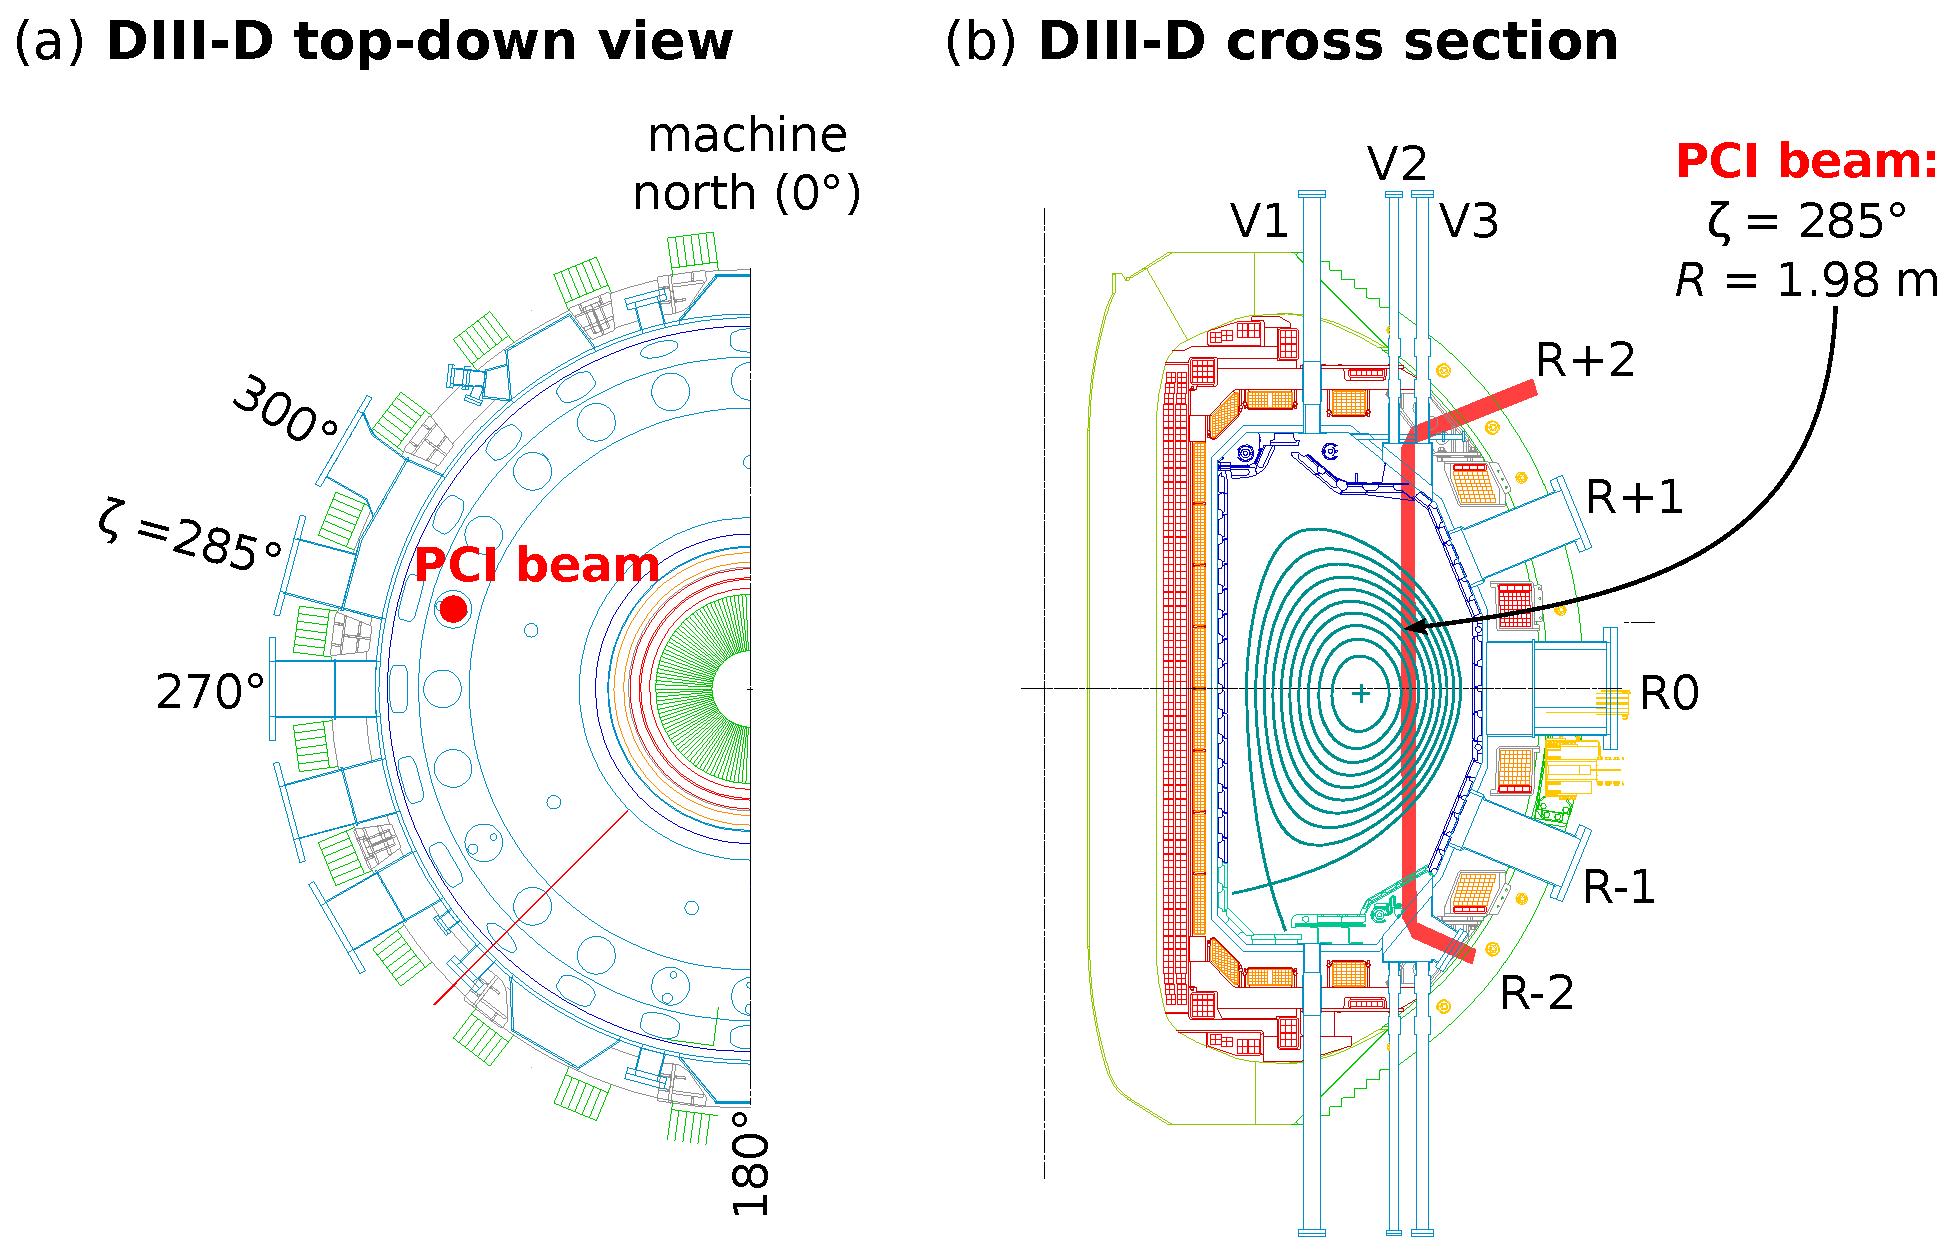
\includegraphics[width = \textwidth]{%
    Chapters/Implementation/figs/d3d_port_locations.eps}
  \caption[\diiid \space port-labeling conventions and location of PCI]{%
    (a) View of \diiid \space from above,
    indicating the toroidal-labeling convention.
    (b) View of \diiid \space cross section,
    indicating the labeling convention
    for vertical (V) and radial (R) sightlines.
    The PCI beam enters the vessel through the $285^{\circ}$ R+2 port,
    propagates vertically downwards through the plasma
    at a major radius of $R = \SI{1.98}{\meter}$, and
    exits the vessel through the $285^{\circ}$ R-2 port.}
\label{fig:Implementation:d3d_port_locations}
\end{figure}


\section{\diiid's pre-existing PCI system}
The \diiid \space PCI system is
thoroughly described elsewhere~\cite{dorris_rsi09}.
The system is currently configured in the ``Phase II'' geometry,
with the probe beam propagating vertically downwards
from the $285^{\circ}$ R+2 to R-2 ports.
The 1/e electric field radius of the in-vessel beam is
$w_0 =$ \SI{3.4}{\centi\meter}, and
the beam center sits at $R = $ \SI{1.98}{\meter}.
A pair of fast steering mirrors dynamically centers
the unscattered beam on the phase plate groove,
compensating for vibrations.
The system has $k_{\text{min}}^{\text{PCI}} = \SI{1.5}{\per\centi\meter}$.

\begin{itemize}
  \item Phase II geometry
  \item $k$-cutoff
  \item Maintenance
    \begin{itemize}
      \item Replacement of laser
      \item Replacement of feedback detector
      \item Replacement of in-vessel mirrors
    \end{itemize}
\end{itemize}

\section{Interferometer design}
\begin{itemize}
  \item Power sharing between the interferometer arms and PCI
  \item TE-cooled detector
  \item Imaging and $k$-response
  \item Demodulation scheme
\end{itemize}

\section{Interferometer optimization}
\begin{itemize}
  \item LO stability
  \item External clock
\end{itemize}

\section{Sound-wave calibration of combined PCI-interferometer}
\begin{itemize}
  \item Importance of speaker placement
  \item System sensitivity
\end{itemize}


\bibliographystyle{plainurl}
\bibliography{references}
